\listfiles
\documentclass[preprint,5p]{elsarticle}
\usepackage[colorlinks=true,linkcolor=blue]{hyperref}%
\usepackage{todonotes}
\usepackage{booktabs}
\usepackage{amssymb}
\usepackage{acronym}
\usepackage{glossaries}
%\usepackage{lineno,hyperref}
%\modulolinenumbers[5]


\journal{None}



%%%%%%%%%%%%%%%%%%%%%%%
%% Elsevier bibliography styles
%%%%%%%%%%%%%%%%%%%%%%%
%% To change the style, put a % in front of the second line of the current style and
%% remove the % from the second line of the style you would like to use.
%%%%%%%%%%%%%%%%%%%%%%%

%% Numbered
%\bibliographystyle{model1-num-names}

%% Numbered without titles
%\bibliographystyle{model1a-num-names}

%% Harvard
%\bibliographystyle{model2-names.bst}\biboptions{authoryear}

%% Vancouver numbered
%\usepackage{numcompress}\bibliographystyle{model3-num-names}

%% Vancouver name/year
%\usepackage{numcompress}\bibliographystyle{model4-names}\biboptions{authoryear}

%% APA style
\bibliographystyle{model5-names}\biboptions{authoryear}

%% AMA style
%\usepackage{numcompress}\bibliographystyle{model6-num-names}

%% `Elsevier LaTeX' style
%\bibliographystyle{elsarticle-num}
%%%%%%%%%%%%%%%%%%%%%%%

\begin{document}

%%%%%%%%%%%%%%%%%%%%%%%%%%%%%%%%%%%%%%
\newcommand{\bookmark}{}

\newcommand{\MinDistance}{1}
\newcommand{\MaxDistance}{7}

\newcommand{\MinDistanceFirst}{1}
\newcommand{\MaxDistanceFirst}{2}

\newcommand{\ns}{[5, 10, 20, 50, 100, 200]}
\newcommand{\nc}{[5, 10, 20, 50, 100, 200]}
\newcommand{\MinDiracs}{25}
\newcommand{\MaxDiracs}{40,000}


\newcommand{\GenerateRepeats}{10}

\newcommand{\nfilters}{8}
\newcommand{\FilterCenter}{70 kHz}

\newcommand{\CorrelationLow}{0.97}
\newcommand{\CorrelationHigh}{$>$ 0.99}

\newcommand{\pcaExplainedVar}{98\%}

\newcommand{\Epochs}{1000}

\newcommand{\FigVIIInumberII}{252}
\newcommand{\FigVIIInumberIII}{63}
\newcommand{\FigVIIInumberIIII}{296}

\newcommand{\Compression}{3-5}

%number of pca components
\newcommand{\pca}{35}
%number of neurons in models
\newcommand{\nneurons}{250 neurons (not including the input and output layers)}
%number of connections
\newcommand{\nweights}{50 thousand}

\newcommand{\noise}{\mathcal{N}}
\newcommand{\noisefloor}{\mathcal{N}_f}
\newcommand{\stochasticnoise}{\mathcal{N}_s}
\newcommand{\db}{dB}


\newacronym{PCA}{PCA}{Principal Component Analysis}
\newcommand{\PCA}{\gls{PCA}} 

\newacronym{pc}{PC}{principal component}
\newcommand{\pc}{\gls{pc}} 
\newcommand{\pcs}{\glspl{pc}} 


%%%%%%%%%%%%%%%%%%%%%%%%%%%%%%%%%%%%%%

\begin{frontmatter}

\title{The low dimensional world of echolocating bats}

%\tnotetext[mytitlenote]{Fully documented templates are available in the elsarticle package on \href{http://www.ctan.org/tex-archive/macros/latex/contrib/elsarticle}{CTAN}.}

%% Group authors per affiliation:
%\author{Elsevier\fnref{myfootnote}}
%\address{Radarweg 29, Amsterdam}
%\fntext[myfootnote]{Since 1880.}

%% or include affiliations in footnotes:
%\author[mymainaddress,mysecondaryaddress]{Elsevier Inc}
%\ead[url]{www.elsevier.com}

%\author[mysecondaryaddress]{Global Customer Service\corref{mycorrespondingauthor}}
%\cortext[mycorrespondingauthor]{Corresponding author}
%\ead{support@elsevier.com}

%\address[mymainaddress]{1600 John F Kennedy Boulevard, Philadelphia}
%\address[mysecondaryaddress]{360 Park Avenue South, New York}

\begin{abstract}
This template helps you to create a properly formatted \LaTeX\ manuscript.
\end{abstract}

%\begin{keyword}
%\texttt{elsarticle.cls}\sep \LaTeX\sep Elsevier \sep template
%\MSC[2010] 00-01\sep  99-00
%\end{keyword}

\end{frontmatter}

%\linenumbers

\section{introduction}

Echolocating bats are long-lived, mobile animals. They use the landscape intensively for foraging, roosting, and commuting. They have excellent spatial memory \citep{Barchi2013,VonHelversen2005} and can rely on sonar to navigate to notable locations like foraging grounds and drinking places \citep[see][for references]{Vanderelst2016,Vanderelst2017}. Bats deprived of sight have been found to successfully return to their roost when displaced by up to 40 miles \citep{Stones1969,Williams1966,Davis1970,Mueller1957}. Furthermore, bats have been reported to use sonar-based recognition of landmarks, both under experimental \citep{Jensen2005,Yu2019}, and natural \citep{Verboom1999} conditions. 

Research on animal navigation has revealed a range of potential strategies that can be used to reach a distant goal \citep[Reviewed by][]{Franz2000}. Irrespective of the strategy an animal uses, a mechanism for recognizing previously visited places is required \citep{Vanderelst2016,Vanderelst2017}. This implies that echolocating bats can identify previously visited sites (or landmarks defining those places) using sonar. Currently, it is still an open question of how bats use sonar to recognize locations in the environment.

One mechanism for place recognition would be for bats to parse the stream of echoes returning from the environment into localized and identified objects \citep{Lee2017,Barchi2013,Moss2001,Schnitzler2003,Simmons2012,Ulanovsky2008,Clare2015,Surlykke2016,Geipel2013}. However, as we argued before, it is highly questionable whether bats can interpret echoes in terms of a 3D environment model or acoustic image \citep[e.g.,][]{Vanderelst2015,Vanderelst2016,Steckel2013}. Sonar projects the three-dimensional structure of the environment on two one-dimensional waveforms arriving at the ears. While the time of arrival of echoes encodes object distance, azimuth and elevation directions are not directly available from the acoustic signal. In principle, azimuth and elevation can be estimated using spectral cues imposed by the head-related transfer function \citep[e.g.,][]{Reijniers2010,Aytekin2004}. However, complex environments, and even single plants \citep{Yovel2008,Muller2000}, return many overlapping and interfering echoes, making reconstructing the direction of origin of echoes much harder, and perhaps impossible. Extracting spatial information is further hampered by the limited temporal resolution of the sonar system \citep{Simmons1989,Wiegrebe1996,Surlykke1996}. 

We have suggested before that limitations of the bat's sonar system result in bats having access to a sparse, low dimensional description of the outside 3D world only \citep{Vanderelst2015a,Vanderelst2016}. Some recent evidence seems to confirm this. First, \citet{Geberl2019} confirmed that bio-sonar has a low spatial resolution, both for distance and angular dimensions. Also, neurophysiological data suggest that closely spaced objects are not perceived separately by echolocating bats. In contrast, neural responses to echo cascades from densely spaced objects seem to represent a single extended stimulus \citep{Warnecke2018,Knowles2015}.

However, it should be noted that such low dimensional descriptions have been shown to contain a lot of useful information \citep{Kuc1997b,Kuc1997} potentially. We previously demonstrated that bats might use sonar template-based scene recognition \citep{Vanderelst2016,Vanderelst2017}. Under this hypothesis, bats compare the acoustic signature of the environment to a set of previously stored signatures. We operationalized these acoustic signatures as time-intensity profiles, which could be derived directly from the cochlear output.

In this paper, we directly evaluate the hypothesis that sonar provides bats inherently with a low dimensional, yet functionally sufficient, description of the world. We test this hypothesis in two steps. In a first step, we generate an extensive collection of synthetic echo sequences. Next, we process the echo sequences using a model of the bat's auditory periphery \citep{Wiegrebe2008}. We assess the compressibility of the output of the cochlear model using \PCA. The synthetic echo sequences differ greatly in complexity. Nevertheless, the output of the cochlear model can be mapped onto a low-dimensional space. In a second step, we show that echoes collected in real bat habitats can be mapped into the same low-dimensional space, without significant loss of information. We verify this by demonstrating that the low dimensional feature space allows recognizing locations in real habitats. 

Together these results suggest that echolocating bats live in a low dimensional perceptual world. The physics of the sonar system and the auditory periphery map the complexity of the 3D environment onto a small number of uncorrelated features, irrespective of whether we use artificial or real echo sequences. Nevertheless, this limited set of features is sufficiently rich for bats to recognize locations, and as we discuss, they could also support flight control.

\section{Methods}

\subsection{Synthetic echoes}

In this section of the paper, we asses how the filtering in the auditory periphery reduces the complexity of input signals. We do this by presenting a simple generative model for echo sequences received by bats. Next, we assess whether the cochlear representation derived from these synthetic echo sequences can be projected into a low dimensional space. 

We created artificial echo sequences by randomly spacing ideal point reflectors. The distances of the point reflectors were selected using a two-step process. First we selected $n_{s}$ seed points $s$, uniformly distributed over a range from \MinDistance\ to \MaxDistance\ meters. Next, for every seed point $s$, we selected $n_{c}$ cloud points normally distributed around $s$, with standard deviation 0.25 m. We added a single reflector at a distance between \MinDistanceFirst\ and \MaxDistanceFirst\ to each collection of points. This two-step process of modeling natural reflectors was inspired by the results of \citet{Yovel2009}, who found that echoes returning from vegetation could be better modeled using a similar two-step process than simply using uniformly spaced points. We generated \GenerateRepeats\ sets of points for each combination of $n_s \in \ns$ and $n_c \in \nc$. Synthetic echoes consisting of few reflectors are likely to consist of only weak echoes.

Each set of points was converted into an environmental impulse response with a sampling frequency $f_s$ of 219 kHz. The environmental impulse response length was set to 7499 samples. These parameters correspond to the recording length and the sampling frequency used in the acoustic data collection (see below). In representing each point reflector by a Dirac impulse, we modeled attenuation of the echoes by introducing an amplitude calculated based on spherical spreading (both ways). The final amplitude of each Dirac impulse was determined by sampling from a normal distribution centered on the calculated amplitude and with a standard deviation of 10 dB. This last operation represents a straightforward model of varying reflector strength due, e.g., to shape and orientation of the reflecting feature.

The impulse responses were converted to echo sequences by convolving them with a bat-like emission. We used a 1 millisecond long linear frequency-swept cosine starting at 100 kHz and ending at 40 Khz. Again, these parameters correspond to those used in the acoustic data collection described below. The echo sequences were dechirped as follows, 
%
%ifft(complex conj(ftt emission) .* fft(echo))
%
\begin{equation}\label{key}
E_d = \mathcal{F}^{-1}((\mathcal{F}(S))^* . \ \mathcal{F}(E))
\end{equation}
with $\mathcal{F}$ denoting the Fourier transform and $()^*$ the complex conjugate. The symbols $S$, $E$, $E_d$ refer to the emission, the echo sequence and the dechirped echo sequence, respectively. Examples of the resulting echo sequences are shown in figures \ref{fig:processing} and \ref{fig:synthetictemplates}. 

Artificial echo sequences were filtered using a model of the bat's auditory periphery, as proposed by \citet{Wiegrebe2008}. This model simulates the temporal and spectral resolution of the bat's cochlea. The model consists of a gammatone filterbank followed by half-wave rectification and non-linear compression with an exponent of 0.4. Finally, the model includes a 1 kHz low-pass filter modeling the response characteristics of the inner hair cells. In the current implementation, we used a gammatone filterbank with \nfilters\ filters, centered around \FilterCenter. The filters were spaced to correspond to equivalent rectangular bandwidths \citep{Glasberg1990}. The output of each channel was attenuated with a time (distance) weighted factor corresponding to the atmospheric attenuation at the channel's center frequency. This operation approximated frequency-dependent atmospheric attenuation. The first 6 ms of data were removed. This was done to ensure the data corresponded with the measurement data. As indicated below, we removed the first 6 ms of the measurement data to avoid including the pickup of the emitted signal. 

Figure \ref{fig:processing}a depicts a single example of a synthetic echo sequence. It also illustrates the resulting response for each of the \nfilters\ channels of the \citet{Wiegrebe2008} model (panels b-i). From these responses, it can be seen that they are highly correlated across channels. This is confirmed when analyzing the average cross-channel correlation for all synthetic echo sequences (Fig. \ref{fig:processing}i). We calculated the correlation $\bar{\rho}$ between the output $X_i$ of each frequency channel $i$ and the mean across channels $\bar{X}$ for each synthetic echo, as follows,
%
\begin{equation}
\bar{\rho} = \frac{1}{n} \sum_i \frac{\mbox{cov}(X_i,\bar{X})}{\sigma_{X_i}, \sigma_{\bar{X}}} 
\end{equation}
%
The distribution of $\bar{\rho}$ is plotted in \ref{fig:processing}j. From this distribution, it can be seen that the value of $\bar{\rho}$ ranged from \CorrelationLow\ to \CorrelationHigh. From these high cross-channel correlations, we conclude that the output of the cochlear model can be summarized by averaging across channels without extensive loss of information. 

An example of such a cross-channel sum is plotted in figure \ref{fig:processing}k. In correspondence to our previous work \citep{Vanderelst2016}, we refer to this average across frequency channels as a template.

\begin{figure*}[tb]
	\centering
	\includegraphics[width=1\linewidth]{../results/processing}
	\caption{Example of synthetic echo sequence and its processing using the \citet{Wiegrebe2008} model. (a) Example of a single synthetic echo sequence (red). The dechirped version is plotted in black. (b-i) Response of the \nfilters\ frequency channels in the \citet{Wiegrebe2008} model. From these plots, it can be seen that channels correlate highly. This is confirmed in panel j, depicting the average correlation across channels for all synthetic echo sequences analyzed. Note that the x-scale does not start at zero. (k) The output of the \citet{Wiegrebe2008} model summed across the frequency channels. This is referred to as a template in this paper. Panel (l) shows the cumulative proportion of explained variance as a function of the number of \pc\ across all templates for all synthetic echo sequences.}
	\label{fig:processing}
\end{figure*}

We used principal components analysis (\PCA\ ) to assess the dimensionality of the templates generated from the synthetic echo sequences. We found that almost all of the variance ($> 99\%$) in the templates could be captured by \pca\ components (see figure \ref{fig:processing}l). Some examples of templates reconstructed from the principal components are shown in figure \ref{fig:synthetictemplates}).

\begin{figure*}[tb]
	\centering
	\includegraphics[width=1\linewidth]{../results/synthetic_templates}
	\caption{Example of synthetic dechirped echo sequences, their corresponding templates and the templates reconstructed from the \pca\ \pcs. (a-c) Three examples of synthetic echo sequence waveforms. Panels (d-f) depict the resulting templates (i.e., summation across the output channels of the \citet{Wiegrebe2008} model). These panels also show the result of projecting the templates into a \pca D \pc\ space and transforming the result back to the original coordinates.}
	\label{fig:synthetictemplates}
\end{figure*}

In this section, we used a generative model for naturalistic echoes. We assumed that echoes sequences received by bats could be considered as generated by anisotropically distributed point reflectors. Using this model, we have derived a low dimensional space ($D = \pca$), which can be used to describe the templates resulting from the artificial echo sequences. This implies that, after filtering through (a model of) the bat's auditory system, these artificial echoes can be converted into low dimensional descriptions. The original echo sequences, generated by \MinDiracs\ to \MaxDiracs\ point reflectors effectively map to a \pca\ dimensional vector. In the remainder of the paper, we will assess whether this low dimensional space allows describing the echoes from real bat habitats as collected using an ensonification device.

\subsection{Natural Templates}

\subsubsection{Acoustic data}

We reused the extensive library of echoes gathered in real bat habitats by \citet{Vanderelst2016}. Below, we briefly discuss the construction of templates based on these echoes, and we refer to our previous work for more details. \citet{Vanderelst2016} constructed an ensonification device featuring 31 Knowles FG series microphones connected to a custom-built sonar data acquisition board \citep{Steckel2013a}. The emitter was a Sensecomp 7000 Series ultrasonic broadband speaker. The ensonification device was mounted on a pan-tilt system allowing to rotate it in azimuth and elevation. The device and pan-tilt system was mounted on a tripod.

\begin{figure}[tb]
	\centering
	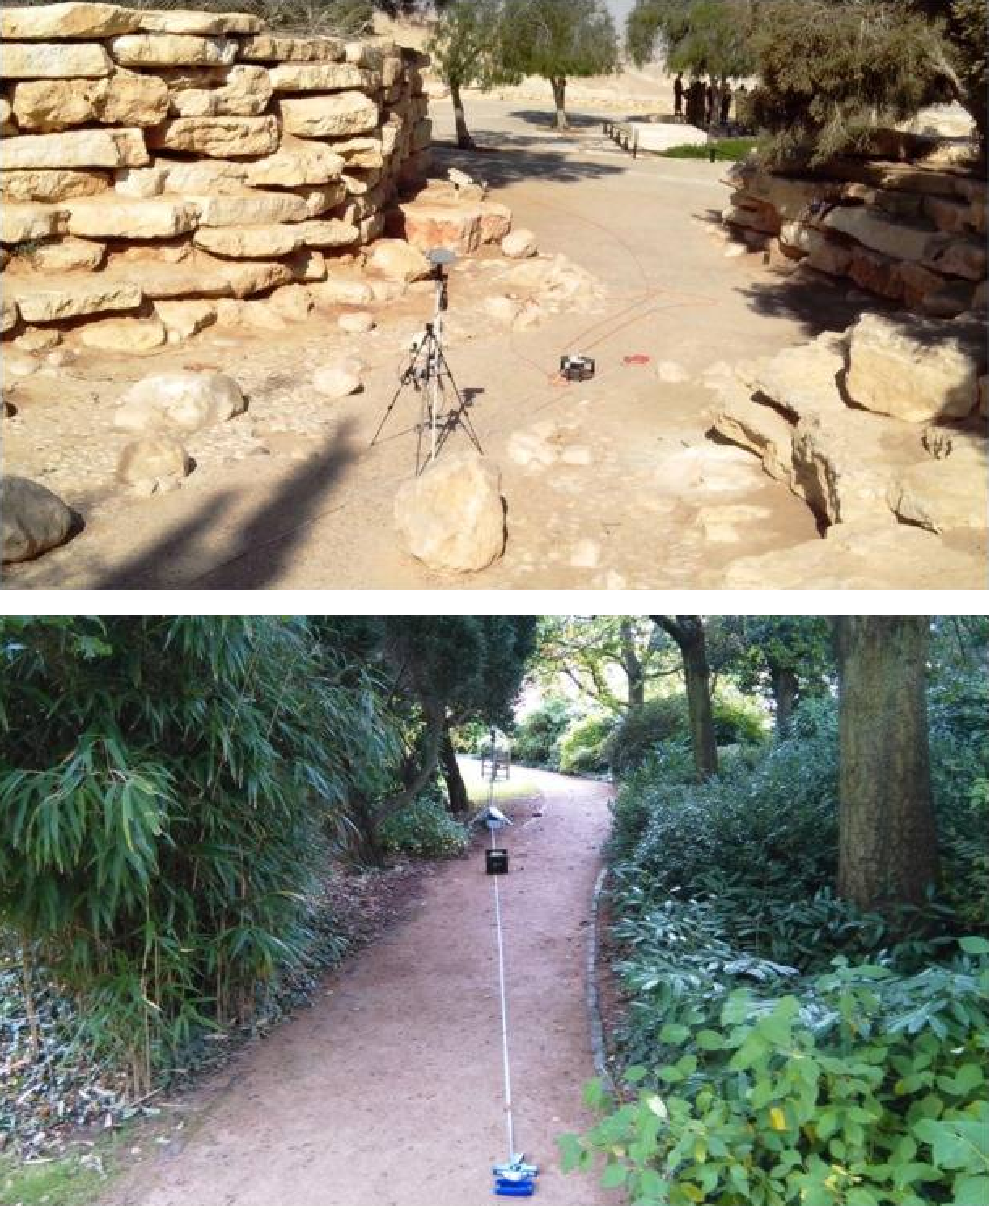
\includegraphics[width=1\linewidth]{figures/datacollection}
	\caption{Pictures of the sonar data acquisition process. Top: the ensonification device used at the Israeli site at Sde Boker. Bottom: The device used at the Bristol University Royal Fort Gardens. The tape measure indicated the transect along which the device was positioned in 40 steps.}
	\label{fig:datacollection}
\end{figure}

Here we use data collected along two linear pathways through natural habitats \citep{Vanderelst2016}. At the first site, a public park in Sde Boker, Israel (Fig. \ref{fig:datacollection}). The environment consisted of a walkway lined with rocks and vegetation. Unpublished bat monitoring data at the site confirmed that bats used this corridor to commute. The ensonification device was placed at 50 positions along a straight line spanning a total of 10 meters Locations were spaced 20 cm apart. At each location, echoes were collected for 31 azimuth directions (-150 to +150 degrees) and 7 elevation directions (-40 to +25 degrees). Therefore, at each location, echoes were collected from 31 x 7 = 217 directions. At each azimuth and elevation direction, three repeat measurements were recorded. In this way, a total of 32,550 echo trains (50 positions x 217 directions x 3 repeats) for each of the 31 microphones in the device were collected.

The second site, at the University of Bristol Royal Fort Gardens (UK), data were collected at 40 different positions along a line (Fig. \ref{fig:datacollection}). Locations were spaced 25 cm apart. As for the Israel site, we collected data for 217 directions, and measurements were repeated three times. This resulted in 26,040 echo trains (40 locations x 217 directions x 3 repeats) for each of 31 microphones. The recording of the echoes started with the emission of a hyperbolic frequency modulated sweep and was recorded for 34 ms ($\sim$5.7 m) at a sampling rate of 219 kHz. 

\subsubsection{Template construction}

For every azimuth and elevation direction at each of the  40 or 50 locations, a biologically plausible acoustic signature of the environment was derived from the echoes, i.e., a template. Below, we briefly outline the steps used to derive templates from the acoustic data.

As we did for the synthetic echo sequences, the echo trains collected in bat habitats were dechirped and filtered using a model of the bat's auditory periphery as proposed by \citet{Wiegrebe2008}. We concluded from analyzing the synthetic echoes that the response in different frequency channels is highly correlated. Therefore, the output of the cochlear model was averaged across frequency channels to obtain a time-intensity profile or template. As the beam of the emitter used was more narrow than the typically combined hearing and emission directionality of bats \citep{Vanderelst2010a,Reijniers2010,Jakobsen2012} templates were averaged across three neighboring directions. The first 6 ms of data were removed to avoid using the emissions themselves for analysis. The processing steps outlined above resulted in 3 $\times$ 217 templates, for each location at each site, corresponding to 217 directions and three repeats.

Among the set of templates, some had very little energy in them, notably those collected for directions without reflectors. For example, aiming the ensonification device upwards often resulted in no echoes returning. These templates could not be classified \citep{Vanderelst2016}. Therefore, we removed them from the current analyses by omitting all templates with very low energy. The resulting number of templates included in the present analyses are given in table \ref{tab:sizes}.

\subsubsection{Noise floor}

Internal (and, potentially, external) noise results in template values greater than zero, even in the absence of reflectors returning echoes. To avoid training the neural network on this noise, we estimated the noise floor in our data by collecting templates while pointing the device to empty space. The maximum template value obtained from these template measurements was used as the noise floor $\noisefloor$. The value of the noise floor $\noisefloor$ used had a numerical value of 0.15. Any template values below this value were set to this value. As we argued before \citep{Vanderelst2016}, using the empirical measurement noise to estimate $\noisefloor$ is biologically warranted as bats have a better signal to noise ratio in their auditory system compared to our measuring device. Indeed, their dynamic range is at least 30 \db\ larger than our measurement device.

\subsubsection{Mapping templates into the \pca-dimensional space}

The templates from both sites were mapped into the \pca-dimensional space derived from the synthetic echoes, described above. We assessed how well templates collected in real habitats could be represented by the \pca\ components by mapping the templates into this space and transforming the results back to the original space. Next, we calculated the correlation (and explained variance) between the original templates and the reconstructed templates.

\subsection{Artificial Neural Networks}

We assessed whether the templates projected into the \pca-dimensional space still contained sufficient information to be recognized. Previously, we assessed whether templates could be used to recognize locations using, what \citet{Baddeley2012} called, a perfect memory approach. Templates were stored in a lookup table. The Euclidean distance between two echo templates was the metric used to assess how well bats should be able to distinguish between templates. This table lookup and distance calculation require a comprehensive search of memory that scales with the number of templates memorized. Hence, in our previous work, we established the theoretical possibility of classifying templates based on real echoes from environments bats were known to frequent, irrespective of the significant amount of memory and computational resources required to do so.  Here, we use a more biologically plausible memory system: an artificial neural network, i.e., a neurally inspired way of distributed information storage \citep{Mcleod1998}. While we acknowledge that current neural network training methods most likely have no biological counterpart, we propose that this approach provides us with a more biologically plausible appraisal of the memory and computational effort required to implement a similar scheme in a bat brain.

Simple artificial feedforward neural networks were implemented using Tensorflow 2 for Python. The first layer of the neural network added Gaussian noise to each input sample ($\sigma(\stochasticnoise) = 0.01$). The following layers were fully connected and used the rectified linear activation function. The output layer uses a softmax activation function, i.e., the normalized exponential function. The loss was calculated as the cross-entropy between the target output and the actual output of the neural network. Weights were updated after each epoch using the Adam algorithm \citep{Kingma2014} .

For each site, we trained three neural networks, each taking the \pca-sample templates as input. The first neural network was trained to output the azimuth direction associated with the template (31 targets). The second network was trained to return the elevation (7 different targets). The final network returned the location (50 or 40 different targets). The targets for the network were encoded using the one-hot encoding scheme. 

Training a different neural network for each of these features ensured that the training algorithm paid equal attention to each feature. When training a single network for all features, the optimization procedure would preferably reduce errors in the location predictions as this feature has the largest variance. The full architecture can be considered as a single network with different streams for each feature (fig. \ref{fig:networks}).

We should point out that we did not take any steps to avoid so-called overfitting by the neural networks. Overfitting occurs when a neural network \citep{Ghotra2017}, or other mathematical models \citep{Hawkins2004}, extract complicated relationships between inputs and outputs that do not hold beyond the training examples. Overfitting typically reduces the ability of the model to generalize its predictive power to new data. However, in this case, the model is not required to generalize to other environments. Instead, we are only interested in whether the neural networks can learn and classify the set of training examples. Nevertheless, it would be beneficial if the neural networks would be capable of classifying templates corresponding to directions that are slightly different from those included in the data sets. Indeed, this is a feature of the Euclidean distance measure used in implementing the perfect memory. In that approach, novel templates will be classified as positions associated with similar templates. We verified whether this property was also found in the neural networks the case by generating a set of templates by interpolating in azimuth and elevation between the directions ensonified in the data set. In our data sets, we ensonified 31 different azimuth directions and seven elevation directions. The interpolated data consisted of 30 azimuths and six elevations. We used the neural networks trained on the original data to classify these interpolated data. 

\begin{figure}
	\centering
	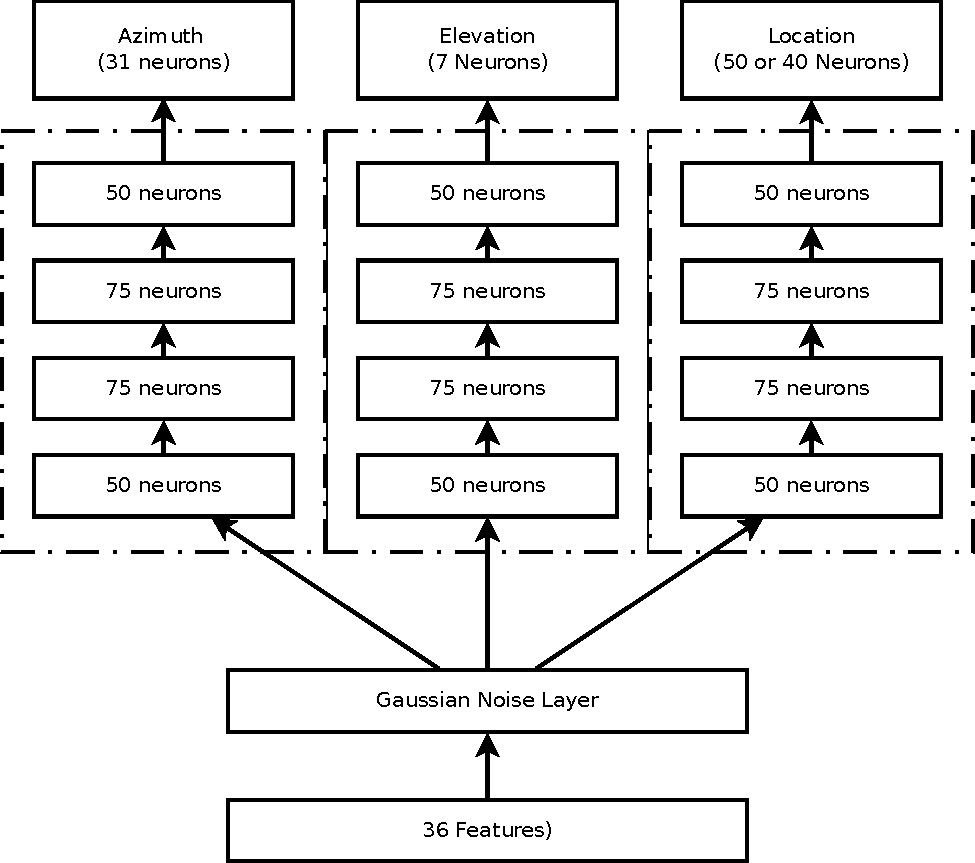
\includegraphics[width=1\linewidth]{figures/networks}
	\caption{Depiction of the neural network architecture trained for each site. The network had 4 hidden layers. The Gaussian Noise Layer adds noise with $\sigma(\stochasticnoise) = 0.01$, as described in the main text.}
	\label{fig:networks}
\end{figure}

\subsubsection{Training examples}

We wished to ensure that the neural networks encoded the templates and were able to recognize them in the presence of realistic noise. Indeed, it can be assumed that neural noise interferes with encoding or memorizing templates. Therefore, we trained the neural networks using templates to which noise was added.

In our previous work, we describe a procedure, based on \citet{Dau1996}, to derive a realistic model for stochastic noise. In brief, we empirically determined a noise level that resulted in a 75\% correct discrimination of two artificial bat calls differing by 2 \db\ in amplitude. This criterion is a conservative estimate of the just noticeable difference in loudness in bats. Based on this procedure we assumed internal (independent) Gaussian stochastic noise $\stochasticnoise$ for each sample with $\sigma(\stochasticnoise) = 0.01$ and $\mu=0$.

\subsection{Perfect Memory}

To be able to directly compare the results of the neural networks with the perfect memory approach \citep{Baddeley2012}, we implemented a version of the classification scheme employed in our earlier work \citep{Vanderelst2016}. We generated noisy templates by adding Gaussian noise to them ($\sigma(\stochasticnoise) = 0.01$). Next, we performed the classification of these noisy templates by finding the closest template (according to the Euclidean distance) in the original set of templates. The location, azimuth, and elevation of the closest template were considered as the noisy template's classification. This was repeated ten times, and we report on the average performance across these repeats.

\section{Results}

We found that the templates derived from acoustic data collected in real habitats could be well represented by the \pca\ components derived from synthetic data. This \pca-dimensional space could represent \pcaExplainedVar\ of the variance in the templates. Figure \ref{fig:empiricaltemplates} shows examples of templates and their reconstructed counterparts. Therefore, although the model used to generate echo sequences was very simple, these results indicate that the \pca D feature space derived from the generative echo model could adequately represent templates resulting from real acoustic data.

\begin{figure*}[tb]
	\centering
	\includegraphics[width=1\linewidth]{../results/empirical_templates}
	\caption{Examples of three templates generated from the echoes collected at the Israel and Royal Fort Gardens site. The panels also depict the result of projecting the templates in the 
		\pca-dimensional space and transforming the result back to the original coordinates.}
	\label{fig:empiricaltemplates}
\end{figure*}

In our previous work \citep{Vanderelst2016}, we showed that the templates could be used to recognize locations in bat habitats. As we have shown that the templates can be projected into a lower \pca D feature space without loss of information, it can be expected that these \pca\ features can be used to recognize locations as well. We found this to be indeed the case.

Figure \ref{fig:history} depicts the training history of all networks. This figure shows that, in all cases, training almost reached an asymptote around or before 250 epochs. However, some additional training can be seen up to \Epochs\ epochs (when learning was arbitrarily halted).

%%
%xx THIS PARAGRAPH TAKES NUMBERS FROM FIG 6
%%

Figure \ref{fig:israelperformance} summarizes the performance of the three neural networks trained on the Israel templates. The performance was obtained by assuming that the most active output neuron represented the classification of the network. Inspecting the cumulative distribution of error reveals that the neural network encoding performed as least as well as the perfect memory approach. The number of small errors was larger for the neural network than for the perfect memory. The neural network was able to classify about 80\% of templates with an error of fewer than 30 degrees in azimuth. In elevation, almost all templates were classified with an error below 15 degrees. Most (78\%) errors in location attribution were smaller than 0.5 meters. The confusion matrices confirm that most classification errors were small.

Interestingly, for azimuth and elevation, classification errors were not uniform across directions. This can be seen by the classification entropy plotted in figure \ref{fig:israelperformance}. In particular, these curves show peaks around zero azimuth and medium elevations. The geometry of the environment can explain these peaks. The corridor (fig. \ref{fig:datacollection}) does not return many echoes from azimuths around zero. Indeed, this direction is mostly open space. The same is true for elevations above 0.

\begin{figure*}
	\centering
	\includegraphics[width=1\linewidth]{../results/israel_results.pdf}
	\caption{Classification results for the Israel site. Top row: cumulative error distributions for the azimuth, elevation and location classification. Middle row: Confusion matrices for the classifications. Bottom row: remaining classification entropy for each target (derived from the confusion matrices).}
	\label{fig:israelperformance}
\end{figure*}

%%
%xx THIS PARAGRAPH TAKES NUMBERS FROM FIG 7
%%

Figure \ref{fig:royalperformance} shows the results for the Royal Fort Park data. These results mirror those in figure \ref{fig:israelperformance}. Again the neural network performed at least as good as the perfect memory approach. For azimuth, the perfect memory approach outperforms the neural network (notice that the y-scale in the top panels of this figure differ from figure \ref{fig:israelperformance}). Overall, the performance for this data set was better than for the Israel data. Probably, this is because echoes were collected closer to reflectors (vegetation) than in the Israel data set, which leads to strong echoes.

\begin{figure*}
	\centering
	\includegraphics[width=1\linewidth]{../results/royal_results.pdf}
	\caption{Classification results for the Royal Fort Park site. Top row: cumulative error distributions for the azimuth, elevation and location classification (Notice the different y-scale for these plots than in figure \ref{fig:israelperformance}). Middle row: Confusion matrices for the classifications. Bottom row: remaining classification entropy for each target (derived from the confusion matrices).}
	\label{fig:royalperformance}
\end{figure*}


\section{Discussion}

\subsection{The low dimensional world of bats}

\citet{Reijniers2010a} quantified the transmission of auditory information in the cochlea of bats. In that study, the authors adapted the Meddis inner hair cell model \citep{Meddis2006} to assess the amount of information in the acoustic signal preserved by the cochlea. The authors concluded that spectral notches introduced by two overlapping echoes are faithfully encoded by auditory nerve spike patterns. However, quantifying the information transfer rate, they also found that about half of the information (in terms of bits) are lost in the transduction from acoustic energy to spike trains. In the current paper, we expand on this work and quantify the dimension reduction due to cochlear encoding. Moreover, we show that this reduction in complexity still supports an ecologically valid task: sonar-based scene recognition.

We assumed echoes received by bats could be modeled as originating from a large collection of point reflectors. Passing these synthetic echoes through a model of the auditory periphery, we obtained a time-intensity profile (template) for each echo sequence. These templates could be well described by a low dimensional space of \pca\ principal components (figure \ref{fig:synthetictemplates}). We found that the same \pca D space could be used to describe templates originating from echoes collected in real bat habitats (figure \ref{fig:empiricaltemplates}). This suggests that the filtering of the auditory periphery provides the bat with a significantly compressed acoustic description of its environment. To identify the locus of the compression, we performed additional analyses. In particular, we evaluated whether the low-dimensional description is a property of the echo sequences themselves, or whether this property results from the finite bandwidths of the gammatone filters or the low-pass filter in the \citet{Wiegrebe2008} model.

We generated templates from the synthetic echo sequences using two versions of the \citet{Wiegrebe2008} model, with and without the 1 kHz low-pass filter. Per default, the model includes this filter to model the response characteristics of the inner hair cells \citep{Meddis2006,Reijniers2010a}. By removing this low-pass filter, we can assess to what extent it is responsible for the observed compressibility of the templates. We also generated templates using echo sequences of which the samples were randomly shuffled. This allows testing whether the templates' low-dimensionality is a property of the echo signals (before being filtered by the cochlear model). 

Figure \ref{fig:mechanism} shows the number of \pcs\ needed to capture 99\% of the templates variance. From this plot, it can be seen that the number of \pcs\ increases when shuffling the echo sequences from \pca\ to \FigVIIInumberIII\. Omitting the 1 kHz filter from the  \citet{Wiegrebe2008} model increases the number of \pcs\ to \FigVIIInumberII. Including the 1 kHz filter, the average spectrum of the templates (fig. \ref{fig:mechanism}, inset) shows that most energy in the templates is contained in frequencies below 1 kHz. Therefore, if we take 1 kHz as the highest relevant frequency, it ought to be possible to completely represent templates by sampling them at 2 kSamples/sec. This corresponds to about 70 samples per template, as templates consist of 7499 samples at 219 kHz sample rate. This corresponds roughly to the number of \pcs\ required to represent templates derived from echo sequences that were shuffled  (fig. \ref{fig:mechanism}). The number of \pcs\ required to represent unshuffled templates is about half of this, i.c., \pca. Therefore, we conclude that the 1 kHz filter is the main, but not exclusive, locus of the dimensionality reduction. The structure of the echo signals also decreases the dimensionality of the templates. The sonar system of bats, through several filtering stages, compresses the 3D complexity of the world onto a lower-dimensional representation.

\begin{figure}[tb]
	\centering
	\includegraphics[width=1\linewidth]{../results/mechanism}
	\caption{Barplot depicting the number of required \pcs\ to capture $>99\%$ of the variance in the templates derived from synthetic echoes. The label \textit{1 kHz filter} refers to whether the 1 kHz filter was omitted in the implementation of the \citet{Wiegrebe2008} model. The label \textit{shuffled} refers to whether the samples of the echoes were randomly shuffled before generating the templates. The inset shows the average spectrum of the templates generated using non-shuffled echoes and a version of the \citet{Wiegrebe2008} model including a 1 kHz filter (i.e., the default model).}
	\label{fig:mechanism}
\end{figure}

Despite the low dimensional character of the templates, they are sufficient to recognize environments. Indeed, this was already demonstrated in our previous work \citep{Vanderelst2016}. Here, we directly demonstrated that the \pca\ principal components are sufficient to discriminate the associated locations and viewing directions using neural networks. The neural networks' performance was somewhat better than the perfect memory approach we used previously (figs. \ref{fig:israelperformance}, \ref{fig:royalperformance}).

While recognizing location in the environment is a critical component of navigation, bats use their sonar not only for navigating. They also rely on sonar for flight control. This includes avoiding obstacles and following guiding structures. The environmental description the bat has access to for flight control starts from the same cochlear output used for place recognition. Therefore, our current work suggests that the same low-dimensional description should be sufficient for flight control as well. Indeed, we have previously demonstrated that a low-dimensional description is sufficient for obstacle avoidance and corridor following \citep{Vanderelst2015a,Mansour2019}. In that work, we converted the echoes at the left and right ear into a template-like representation. We used this representation as input to the robot controller. Subsequent work will have to demonstrate whether the parameters of the \pca D space presented here can be used directly for controlling flight. In other words, we conjecture it should be possible to extract \pca\ features from an echo signal and convert this vector into a motor command. One could presume a neural network that converts the \pca\ features to flight control parameters.

\subsection{Template encoding}

We were unable to find values for the number of neurons in the cortex of bat species. However, the mouse cortex has been estimated to contain about $9 \cdot 10^4$ neurons or $7 \cdot 10^8$ synapses per cubic millimeter \citep{Braitenberg2013}. The neural networks presented in this paper consisted of \nneurons\ and \nweights\ connections. Therefore, to the extent that the proposed neural networks can be considered as biologically plausible models of memory, they are orders of magnitude smaller than a single cubic millimeter of mouse cortex. Let alone the complete cortex, which has been estimated to contain 75 million neurons \citep{Williams2000}. 

Despite their small size, the neural networks were able to encode (memorize) the templates at least as well as the perfect memory approach. The neural networks presented here are tiny compared to the density of cortical matter. However, the networks are also small compared to the data they encode. Table \ref{tab:sizes} lists the number of weights for the artificial neural networks and compares this number with the size of the \pca-dimensional templates. The number of floating-point numbers making up the templates is larger than the number of weights by a factor of \Compression. Therefore, the networks have a smaller memory footprint than the data they encode. It should be noted that we have not attempted to try and to optimize (minimize) the size of the networks. From these numbers, we conclude that the low-dimensional signals provided by the bat's sonar system result in a low memory footprint and that they would use limited neural resources to be stored and processed.

\begin{table}
	\centering
	\begin{tabular}{lrrrrl}
		\toprule
		Site &       T &     n &      W &  W (nb) &      R \\
		\midrule
		Israel &  183430 &  5395 &  52875 &   51975 &  28.8\% \\
		Royal &  264146 &  7769 &  51345 &   50475 &  19.4\% \\
		\bottomrule
	\end{tabular}
	\label{tab:sizes}
	\caption{Table indicating the size of both template data sets and the number of weights in the networks. The template size $T$ is obtained as $\pca \times n$, with $n$ the number of templates in the set. The number of weights $W$ includes all connections between neurons and the bias weights. $W (nb)$ omits the bias weights. The ratio $R$ gives the ratio $W/T$.}
\end{table}


\subsection{Conclusion}

It has been suggested that bats' sonar systems provide detailed information about the world. Several authors have referred to sonar as providing the bat with an acoustic image \citep{Lee2017,Barchi2013,Moss2001,Schnitzler2003,Simmons2012,Ulanovsky2008,Clare2015,Surlykke2016,Geipel2013}. As mentioned above, this is at odds with some recent behavioral and neurophysiological findings in bats faced with complex echo sequences \citep{Knowles2015,Geberl2013,Warnecke2018}. However, it is also at odds with the various filtering stages involved in the emission and the reception of bio-sonar. In particular, we argued before that the neurophysiology of the bats' auditory system represents a bottleneck in the amount of raw echo signal information accessible to the bat. Indeed, \citet{Reijniers2010a} already noticed that significant compression occurs during cochlear transduction. Here, we followed up on that work to quantify the dimensional reduction of the input signals as a result of peripheral auditory processing.

From our current work, in combination with previous results \citep{Vanderelst2016,Vanderelst2015a,Mansour2019,Reijniers2010a}, we conclude that the sonar system of bats maps complex echo signals onto a limited number of features. These features can be efficiently stored to recognize scenes. Moreover, we conjecture that a (binaural) version of the features should allow for sonar-based flight control. As such, a view of echolocating bats living in a low dimensional sensory space emerges that is at odds with the widespread notion of sonar as a sensing modality that provides detailed acoustic images.

\bibliography{references}

\onecolumn
\appendix
\section{Supplementary material}

\begin{figure}[h]
	\centering
	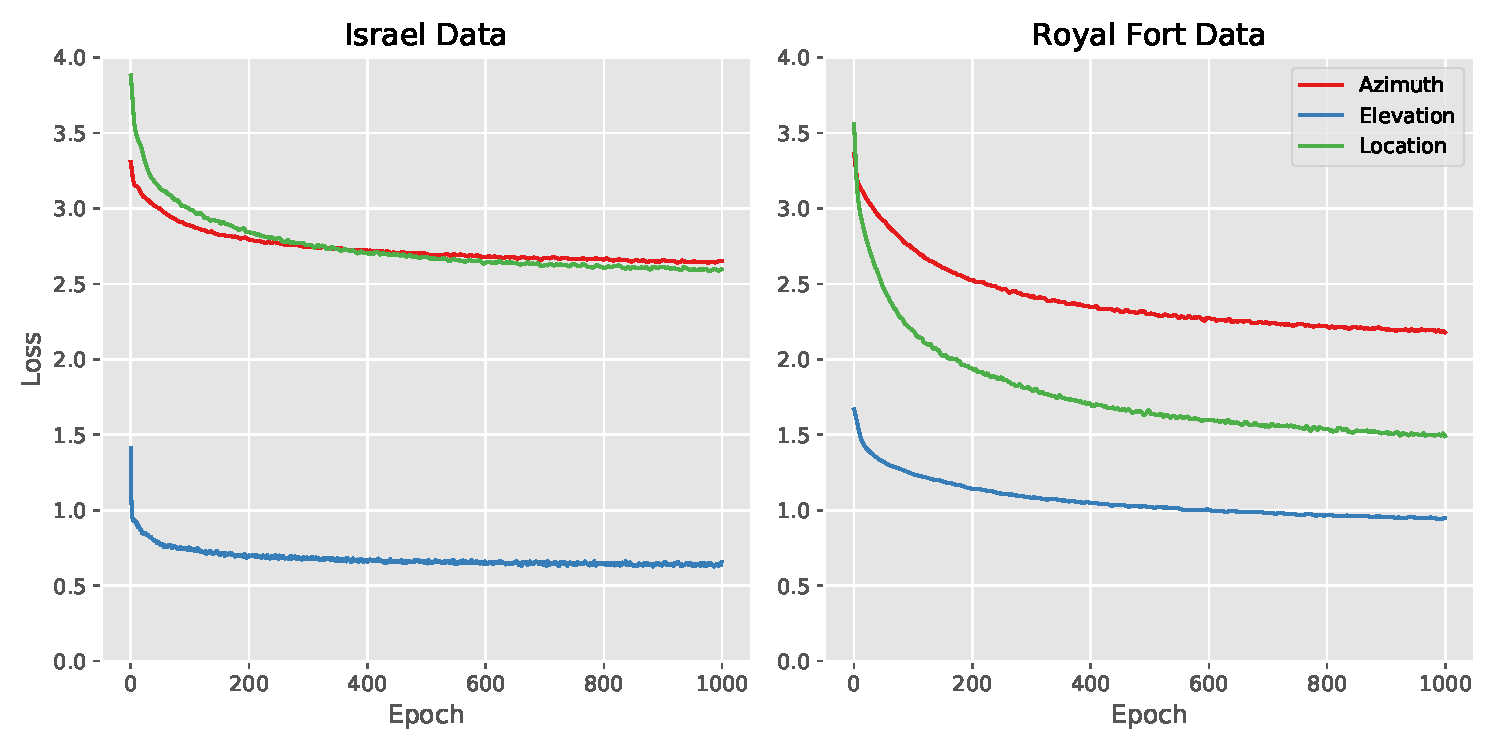
\includegraphics[width=1\linewidth]{../results/history}
	\caption{Training history of the neural networks. The plots give the value of the loss function as a function of training epoch. Notice the logarithmic x-axis.}
	\label{fig:history}
\end{figure}

\begin{figure}[h]
	\centering
	\includegraphics[width=1\linewidth]{../results/components}
	\caption{Plot of the first 25 \pcs\ (out of \pca). The number in each panel indicates the number of zero crossings in the template. This number increases as a function of template number, indicating that most information is contained in lower template frequencies.}
	\label{fig:components}
\end{figure}

\begin{figure}[h]
	\centering
	\includegraphics[width=1\linewidth]{../results/interpolation}
	\caption{Neural network categorization results for the templates obtained by interpolating between the seven elevation and 31 azimuth directions ensonified for the Israel and Royal Fort site. (a,b) results for the azimuth and elevation for the Israel data. (c,d) Same for the Royal Fort data. Because the templates classified in these results were interpolated, the network can be considered to have correctly classified the template if it is assigned to direction $n$ or direction $n+1$. For example, a template obtained by interpolating between azimuth directions 140 and 130 degrees could be assigned to either these directions. The number in each panel indicates the percentage of data point on the diagonal (direction $n$) or the diagonal + 1 ($n+1$).}
	\label{fig:interpolation}
\end{figure}


\end{document}
